% PaperTrade ER diagram (CSC 370)
% Notation: entity = rectangle, weak entity = double rectangle,
% relationship = diamond, identifying relationship = double diamond,
% attribute = oval, key = underlined oval, partial key = dashed underline.
\documentclass[border=10pt]{standalone}
\usepackage{tikz}
\usetikzlibrary{er,positioning,arrows.meta}

\begin{document}
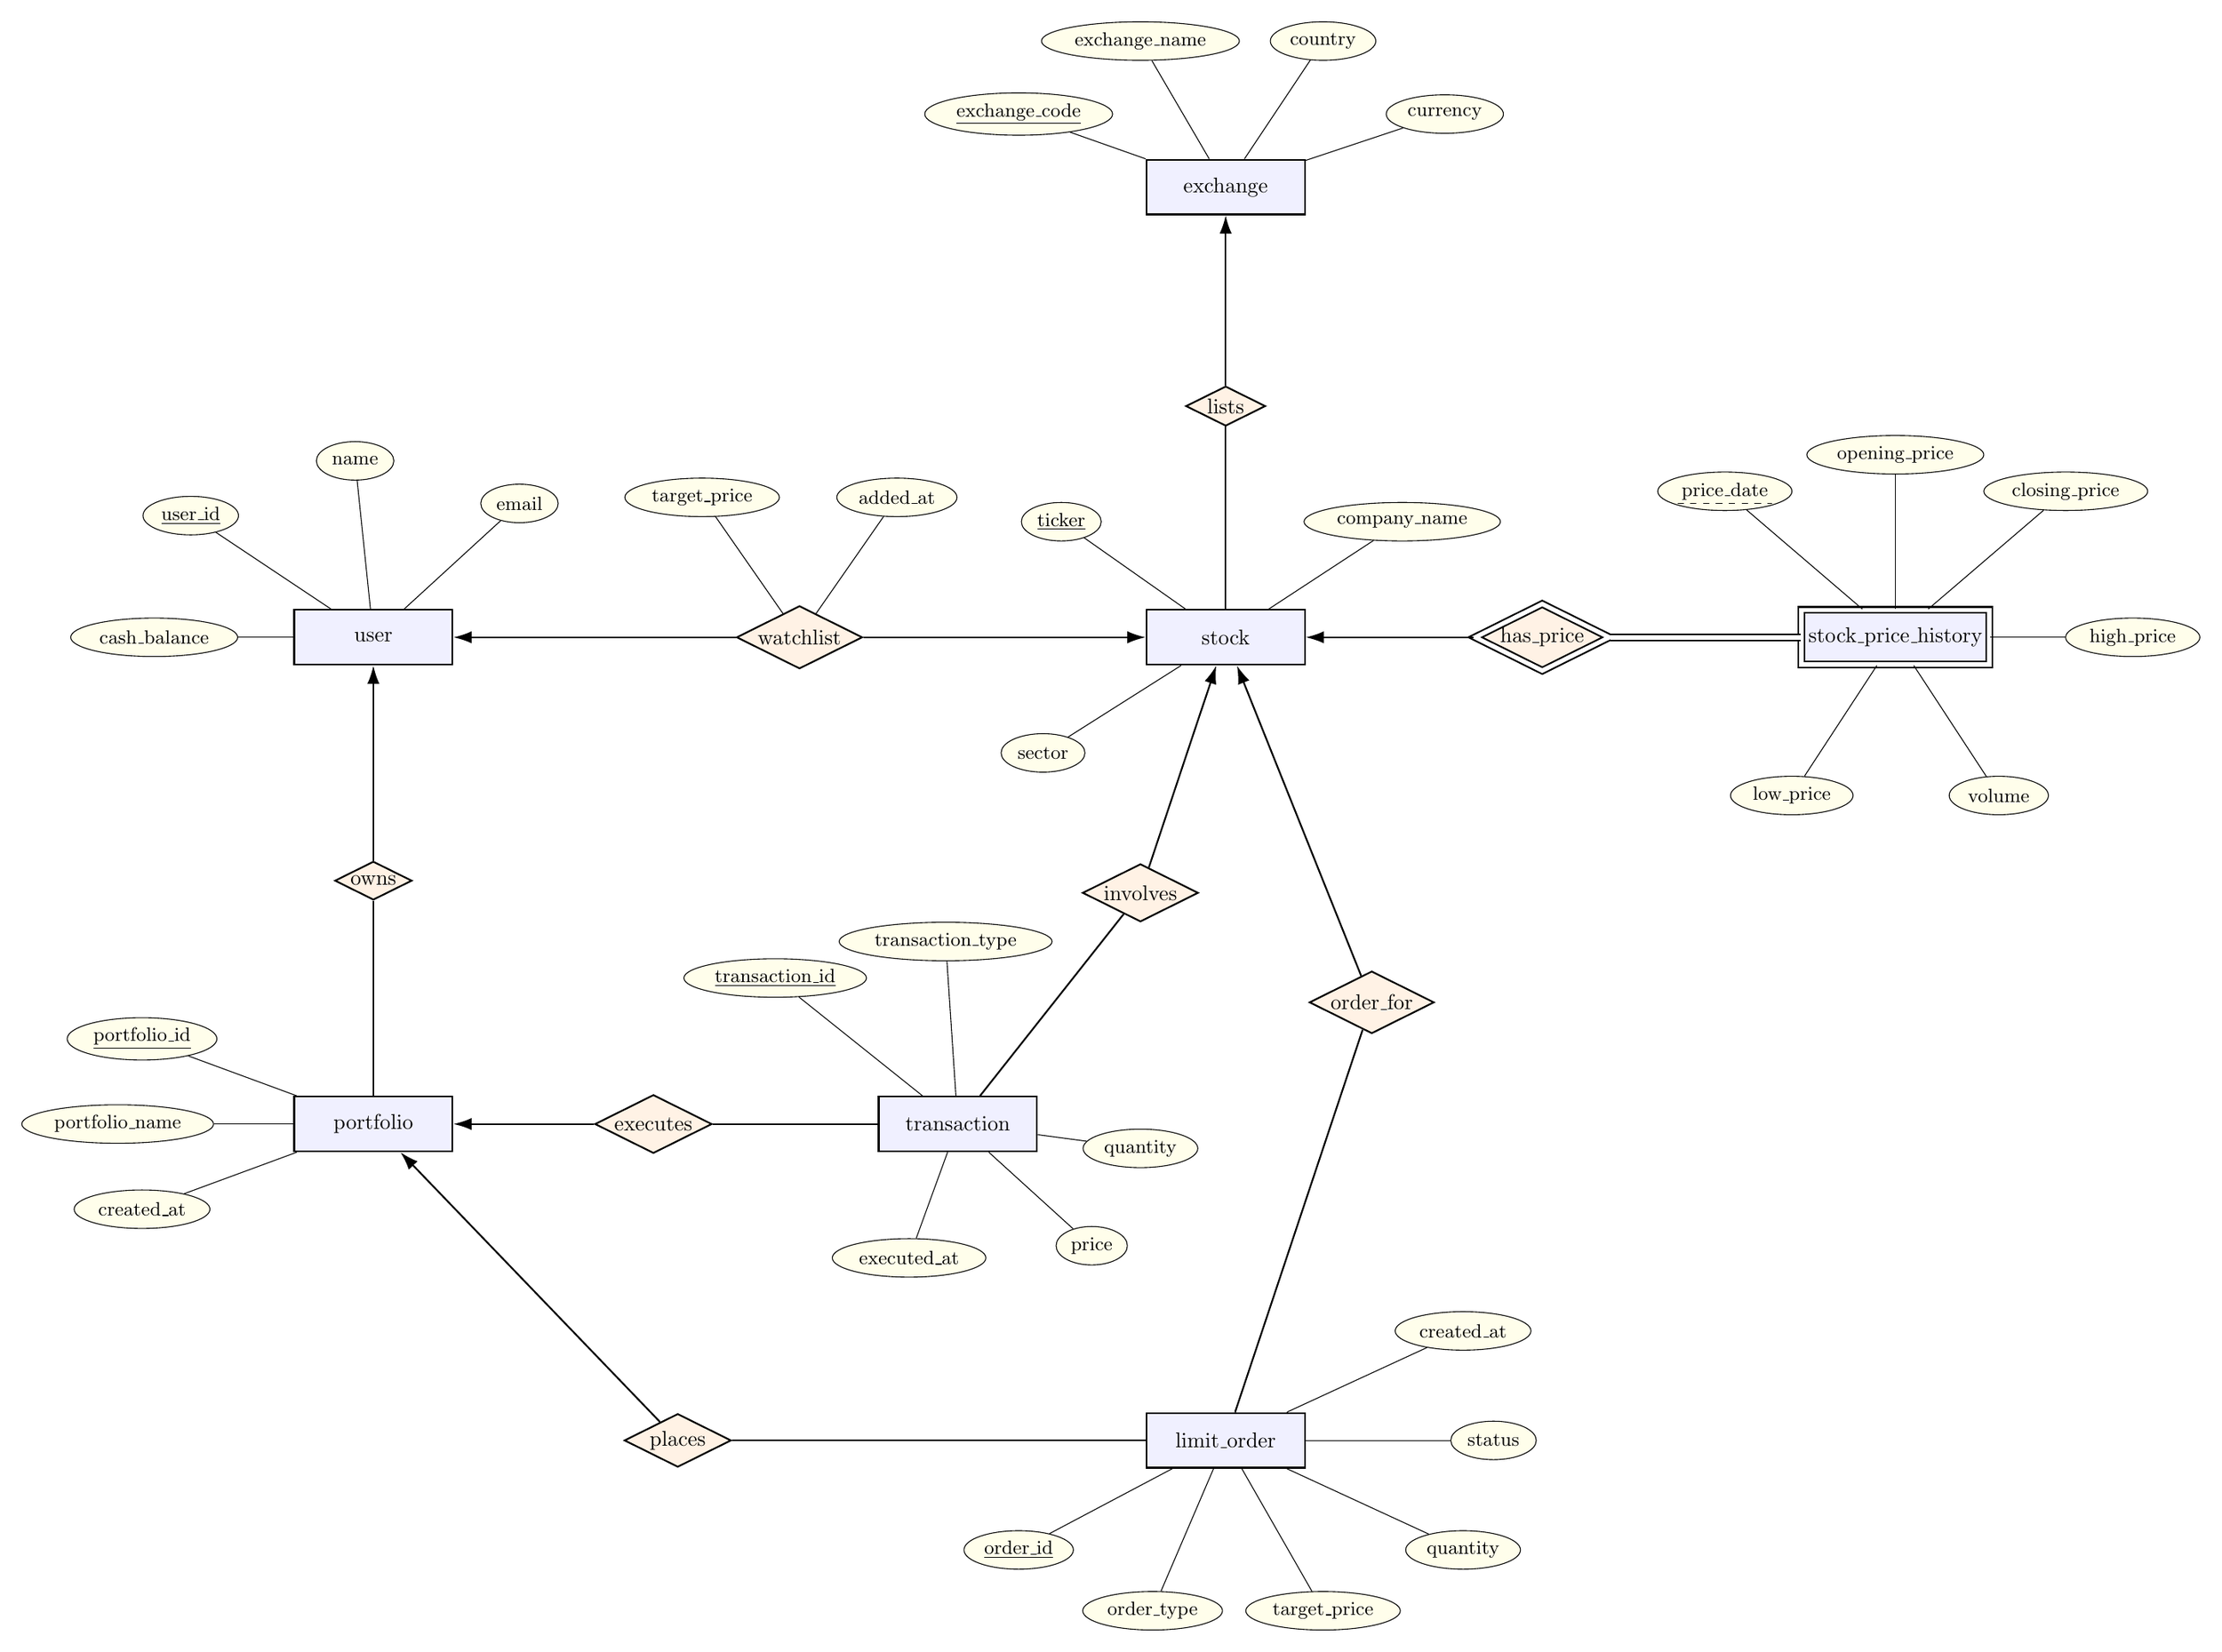
\begin{tikzpicture}[
    auto,
    every entity/.style={draw, thick, minimum width=2.6cm, minimum height=0.9cm, fill=blue!6},
    every relationship/.style={draw, thick, aspect=2, fill=orange!10, inner sep=1pt},
    every attribute/.style={draw, fill=yellow!8, inner sep=2pt, font=\small},
    every edge/.style={draw, thick},
    card/.style={font=\small\bfseries, inner sep=2pt},
    % the er library in some TeX distributions lacks these, so define them here
    weak entity/.style={entity, double, double distance=2pt},
    ident relationship/.style={relationship, double, double distance=2pt},
    total/.style={double, double distance=2pt},
    % arrowhead points at the entity on the "one" side (M:N gets both, 1:1 none)
    one/.style={-{Latex[length=3mm,width=2mm]}},
    % partial key (discriminator) of a weak entity: dashed underline
    partial key/.style={attribute, path picture={
        \draw[dashed] ([xshift=-0.78cm,yshift=-0.2cm]path picture bounding box.center)
                    -- ([xshift=0.78cm,yshift=-0.2cm]path picture bounding box.center);}},
  ]

  % ===================== USER =====================
  \node[entity] (user) at (0,0) {user};
  \node[attribute] (u1) at (-3.0, 2.0) {\underline{user\_id}};
  \node[attribute] (u2) at (-0.3, 2.9) {name};
  \node[attribute] (u3) at ( 2.4, 2.2) {email};
  \node[attribute] (u4) at (-3.6, 0.0) {cash\_balance};
  \foreach \a in {u1,u2,u3,u4} \draw (user) -- (\a);

  % ===================== PORTFOLIO =====================
  \node[relationship] (owns) at (0,-4) {owns};
  \node[entity] (portfolio) at (0,-8) {portfolio};
  \node[attribute] (p1) at (-3.8,-6.6) {\underline{portfolio\_id}};
  \node[attribute] (p2) at (-4.2,-8.0) {portfolio\_name};
  \node[attribute] (p3) at (-3.8,-9.4) {created\_at};
  \foreach \a in {p1,p2,p3} \draw (portfolio) -- (\a);

  \path (owns) edge[one] (user)
               edge (portfolio);

  % ===================== WATCHLIST (M:N) =====================
  \node[relationship] (watch) at (7,0) {watchlist};
  \node[attribute] (w1) at (5.4, 2.3) {target\_price};
  \node[attribute] (w2) at (8.6, 2.3) {added\_at};
  \foreach \a in {w1,w2} \draw (watch) -- (\a);

  % ===================== STOCK =====================
  \node[entity] (stock) at (14,0) {stock};
  \node[attribute] (s1) at (11.3, 1.9) {\underline{ticker}};
  \node[attribute] (s2) at (16.9, 1.9) {company\_name};
  \node[attribute] (s3) at (11.0,-1.9) {sector};
  \foreach \a in {s1,s2,s3} \draw (stock) -- (\a);

  \path (watch) edge[one] (user)
                edge[one] (stock);

  % ===================== EXCHANGE =====================
  \node[relationship] (lists) at (14,3.8) {lists};
  \node[entity] (exchange) at (14,7.4) {exchange};
  \node[attribute] (e1) at (10.6, 8.6) {\underline{exchange\_code}};
  \node[attribute] (e2) at (12.6, 9.8) {exchange\_name};
  \node[attribute] (e3) at (15.6, 9.8) {country};
  \node[attribute] (e4) at (17.6, 8.6) {currency};
  \foreach \a in {e1,e2,e3,e4} \draw (exchange) -- (\a);

  \path (lists) edge[one] (exchange)
                edge (stock);

  % ===================== STOCK_PRICE_HISTORY (weak) =====================
  \node[ident relationship] (hasprice) at (19.2,0) {has\_price};
  \node[weak entity] (sph) at (25,0) {stock\_price\_history};
  \node[partial key] (h1) at (22.2, 2.4) {price\_date};
  \node[attribute] (h2) at (25.0, 3.0) {opening\_price};
  \node[attribute] (h3) at (27.8, 2.4) {closing\_price};
  \node[attribute] (h4) at (28.9, 0.0) {high\_price};
  \node[attribute] (h5) at (23.3,-2.6) {low\_price};
  \node[attribute] (h6) at (26.7,-2.6) {volume};
  \foreach \a in {h1,h2,h3,h4,h5,h6} \draw (sph) -- (\a);

  \path (hasprice) edge[one] (stock);
  \path (hasprice) edge[total] (sph);

  % ===================== TRANSACTION =====================
  \node[relationship] (executes) at (4.6,-8) {executes};
  \node[entity] (trans) at (9.6,-8) {transaction};
  \node[attribute] (t1) at ( 6.6,-5.6) {\underline{transaction\_id}};
  \node[attribute] (t2) at ( 9.4,-5.0) {transaction\_type};
  \node[attribute] (t3) at (12.6,-8.4) {quantity};
  \node[attribute] (t4) at (11.8,-10.0) {price};
  \node[attribute] (t5) at ( 8.8,-10.2) {executed\_at};
  \foreach \a in {t1,t2,t3,t4,t5} \draw (trans) -- (\a);

  \path (executes) edge[one] (portfolio)
                   edge (trans);

  \node[relationship] (involves) at (12.6,-4.2) {involves};
  \path (involves) edge (trans)
                   edge[one] (stock);

  % ===================== LIMIT_ORDER =====================
  \node[relationship] (places) at (5.0,-13.2) {places};
  \node[entity] (lorder) at (14,-13.2) {limit\_order};
  \node[attribute] (l1) at (10.6,-15.0) {\underline{order\_id}};
  \node[attribute] (l2) at (12.8,-16.0) {order\_type};
  \node[attribute] (l3) at (15.6,-16.0) {target\_price};
  \node[attribute] (l4) at (17.9,-15.0) {quantity};
  \node[attribute] (l5) at (18.4,-13.2) {status};
  \node[attribute] (l6) at (17.9,-11.4) {created\_at};
  \foreach \a in {l1,l2,l3,l4,l5,l6} \draw (lorder) -- (\a);

  \path (places) edge[one] (portfolio)
                 edge (lorder);

  \node[relationship] (orderfor) at (16.4,-6.0) {order\_for};
  \path (orderfor) edge (lorder)
                   edge[one] (stock);

\end{tikzpicture}
\end{document}
